\chapter{Evaluation}
\label{cha:evaluation}
For evaluation purposes, 6LoCAN is implemented in the Zephyr RTOS network stack.

\begin{table}[htp]
	\centering
	\caption{Resource demand of 6LoCAN}
	\begin{tabular}{|l|r|r|} \hline
        \makecell[c]{Layer}   & \makecell[c]{RAM} & \makecell[l]{ROM} \\ \hline \hline
        CAN Driver            & 256   & 3878 \\ \hline
        Network CAN Driver    & 328   & 1354 \\ \hline
        IPHC                  & 4     & 2779 \\ \hline
        6LoCAN                & 1664  & 6534 \\ \hline
        \makecell[l]{Networking\\(incl. 6LoCAN, without drivers)} & 34016 & 57269 \\ \hline
	\end{tabular}
	\label{tab:resources}
\end{table}

\autoref{tab:resources} shows the RAM and ROM demand of the 6LoCAN implementation.
The build is the echo\_server sample application, built on Zephyr 2.2 with 6LoCAN enabled.
It includes the IPv6 network stack, TCP, and UDP.
The sample uses 64 net buffers for each, receiving and sending.
One buffer can hold up to 128 bytes, which results in 8192 bytes for sending and 8192 bytes for sending.
As shown in the table, the 6LoCAN does not add an excessive amount of RAM and ROM.
The sample uses 64 net buffers each, for receiving and sending.
As shown in the table, the 6LoCAN does not add an excessive amount of RAM and ROM.
Most of the RAM is used for the sending and receiving buffers.
The 6LoCAN contexts use 1024 of the 1664 bytes of RAM.
The ROM overhead of 6LoCAN in the entire network stack is only 11.4 \%.

\begin{figure}[htp]
	\begin{center}
	\begin{tikzpicture}[
		scale=0.8,
		every node/.append style={scale=0.8},
		can_node/.style={
			align=center,
			fill=blue!5,
			rectangle,
			draw=black,
			rounded corners=0.1cm,
			minimum width = 3.5cm,
			minimum height = 5cm,
			node distance=1cm},
		can_trans/.style={
			align=center,
			fill=black!5,
			rectangle,
			draw=black,
			rounded corners=0.1cm,
			minimum width = 2.5cm,
			minimum height = 2cm,
			node distance=1.25cm},
		host_node/.style={
			align=center,
			fill=green!5,
			rectangle,
			draw=black,
			rounded corners=0.1cm,
			minimum width = 3.5cm,
			minimum height = 5cm,
			node distance=2cm},
		logicanalyzer/.style={
			align=center,
			fill=green!5,
			rectangle,
			draw=black,
			rounded corners=0.1cm,
			minimum width = 3.5cm,
			minimum height = 2cm,
			node distance=4cm}
		]

		\node (node1)[can_node] {STmicro\\Nucleo-F746ZG};
		\node (trans1)[can_trans, above = of node1] {CAN\\Transceiver};
		\node (node2)[can_node, right = of node1] {NXP\\FRDM-K64F};
		\node (trans2)[can_trans, above = of node2] {CAN\\Transceiver};
		\node (node3)[can_node, right = of node2] {STmicro\\Nucleo-F746ZG};
		\node (trans3)[can_trans, above = of node3] {CAN\\Transceiver};
		\node (host)[host_node, below = of node1] {Host-PC};
		\node (logicanalyzer)[logicanalyzer, right = of host, yshift=-1.5cm] {Logic-Analyzer};

		\draw ([xshift=1cm]trans1.north) -- ++(0,1cm) node[above, xshift=0.75cm]{GND} -|  ([xshift=1cm]trans3.north);
		\draw ([xshift=1cm]trans2.north) -- ++(0,1cm);
		\draw ([xshift=-0.25cm]trans1.north) -- ++(0,2.5cm) node[above, xshift=2cm]{CAN H} -|  ([xshift=-0.25cm]trans3.north);
		\draw ([xshift=-0.25cm]trans2.north) -- ++(0,2.5cm);
		\draw ([xshift=0.25cm]trans1.north) -- ++(0,2cm) node[above, xshift=1.5cm]{CAN L} -| ([xshift=0.25cm]trans3.north);
		\draw ([xshift=0.25cm]trans2.north) -- ++(0,2cm);
		\foreach \i in {1,2,3}{
			\draw[<-] ([xshift=-0.75cm]trans\i.south) -- ([xshift=-0.75cm]node\i.north) node[midway, above, rotate=90] {TX};
			\draw[->] ([xshift=-0.25cm]trans\i.south) -- ([xshift=-0.25cm]node\i.north) node[midway, above, rotate=90] {RX};
			\draw ([xshift=0.25cm]trans\i.south) -- ([xshift=0.25cm]node\i.north) node[midway, above, rotate=90] {5V};
			\draw ([xshift=0.75cm]trans\i.south) -- ([xshift=0.75cm]node\i.north) node[midway, above, rotate=90]  {GND};
		}

		\draw ([xshift=-1cm]node1.south) -- ([xshift=-1cm]host.north) node[midway, anchor=east] {USB};
		\draw ([xshift=-1cm]node2.south) |- ([yshift=1.5cm]host.east) node[midway, anchor=west] {USB};
		\draw ([xshift=-1cm]node3.south) |- ([yshift=1cm]host.east) node[midway, anchor=west] {USB};

		\draw (node1.south) -- (host.north) node[midway, anchor=west] {Ethernet};

		\draw (logicanalyzer.west) -- (host.east |- logicanalyzer.west) node[midway, above] {USB};
		\draw[<-] ([yshift=-0.25cm]logicanalyzer.east) -- ++(2cm,0) node[midway, below] {CAN RX} |- ([xshift=-0.25cm, yshift=-0.25cm]trans3.south);
		\draw ([yshift=0.25cm]logicanalyzer.east) -- ++(1.5cm,0) |- ([xshift=0.75cm, yshift=-1cm]trans3.south);
	
	\end{tikzpicture}
	\caption{Test Setup}
	\label{fig:eval_setup}
	\end{center}
\end{figure}


\autoref{fig:eval_setup} shows the setup used for all evaluated data in this section.
USB is used as a power supply and provides a UART terminal.
The boards are flashed with an application that transfers data when issuing a command over UART.
The boards are connected to the CAN-bus with a CAN-transceiver. One board also has Ethernet, connected to the host.
This Ethernet port serves as the Boarder-Translator.
The Logic-Analyzer is used to determine the exact timing of the frames.

\subsection{Link-Layer Duplicate Address Detection}

\begin{figure}[htp]
        \begin{center}
                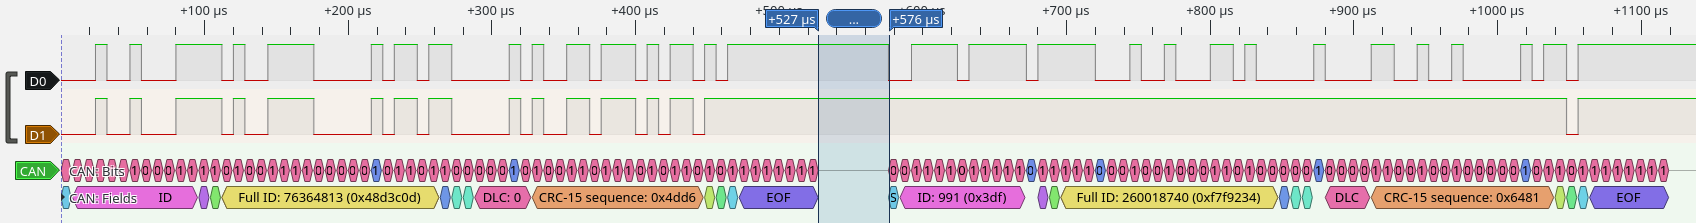
\includegraphics[width=\textwidth]{figures/eval_dad_logic.png}
        \end{center}
        \caption{Link-Layer Duplicate Address Detection Measurement}
        \label{fig:eval_lldad}
\end{figure}

Two boards are programmed with the same fixed address (0x1234) to evaluate the Link-Layer Duplicate Address Detection.
\autoref{fig:eval_lldad} shows a capture of the LLDAD.
The black trace is the CAN\_RX line and therefor shows the logic levels on the bus.
The brown trace is the CAN\_TX line and, therefore, only shows the data sent by the node that issues the LLDAD.
The first CAN frame is the LLDAD request. The identifier used is 0x48d3c0d (DST: 0x1234, SRC (entropy): 0x3C0D) and the RTR bit is set.
The second frame is the response from the other node, already using the same address.
The identifier is 0xf7f9234 (DST: 3DEF, SRC: 0x1234).
The node that caused the address duplication noticed the duplication and disabled the interface.

\begin{lstlisting}[numbers=none, basicstyle=\tiny]
[00.001] <inf> net_l2_canbus: DAD failed

Interface 0x2002dde0 (CANBUS) [1]
=================================
Interface is down.
\end{lstlisting}
\newpage

\subsection{Ping}
This section shows the evaluation of a Ping command.
One board has a fixed address of 0x1234, and the other board has a randomly chosen address.
The logs below show what is going on during the brin up of the interface and pings.

First node with the address 0x1234:
\begin{lstlisting}[numbers=none, basicstyle=\tiny]
=================================== Interface bring up ===================================
[00.471] Sending  Multicast Listener Report v2 type 143 code 0 from :: to ff02::16
[00.471] Sending  Multicast Listener Report v2 type 143 code 0 from :: to ff02::16
[00.471] Sending  Neighbor Solicitation type 135 code 0 from :: to ff02::1:ff00:1234 <-(DAD)
[00.472] Sending  Router Solicitation   type 133 code 0 from :: to ff02::1
[01.472] Sending  Router Solicitation   type 133 code 0 from fe80::ff:fe00:1234 to ff02::1
[01.479] Router Solicitation received   type 133 code 0 from fe80::ff:fe00:314e to ff02::1
[02.472] Sending  Router Solicitation   type 133 code 0 from fe80::ff:fe00:1234 to ff02::1
[02.479] Router Solicitation received   type 133 code 0 from fe80::ff:fe00:314e to ff02::1
==========================================================================================

======================= Start of the Neighbor Dicovery from the pinging node ========================
[03.577] Neighbor Solicitation received  type 135 code 0 from fe80::ff:fe00:314e to ff02::1:ff00:1234
[03.577] Sending  Neighbor Solicitation  type 135 code 0 from fe80::ff:fe00:1234 to ff02::1:ff00:314e
[03.577] Sending Neighbor Advertisement  type 136 code 0 from fe80::ff:fe00:1234 to fe80::ff:fe00:314e
[03.600] Neighbor Solicitation received  type 135 code 0 from fe80::ff:fe00:314e to ff02::1:ff00:1234
[03.600] Sending Neighbor Advertisement  type 136 code 0 from fe80::ff:fe00:1234 to fe80::ff:fe00:314e
[03.609] Neighbor Advertisement received type 136 code 0 from fe80::ff:fe00:314e to fe80::ff:fe00:1234
======================================================================================================

=========================================== Pings ==========================================
[03.618] Echo Request received type 128 code 0 from fe80::ff:fe00:314e to fe80::ff:fe00:1234
[03.618] Sending Echo Reply    type 129 code 0 from fe80::ff:fe00:1234 to fe80::ff:fe00:314e
[04.573] Echo Request received type 128 code 0 from fe80::ff:fe00:314e to fe80::ff:fe00:1234
[04.574] Sending Echo Reply    type 129 code 0 from fe80::ff:fe00:1234 to fe80::ff:fe00:314e
[05.574] Echo Request received type 128 code 0 from fe80::ff:fe00:314e to fe80::ff:fe00:1234
[05.574] Sending Echo Reply    type 129 code 0 from fe80::ff:fe00:1234 to fe80::ff:fe00:314e
============================================================================================
\end{lstlisting}

Second node with the address 0x314e:
\begin{lstlisting}[numbers=none, basicstyle=\tiny]
=================================== Interface bring up ==================================
[00.101] Sending Multicast Listener Report v2 type 143 code 0 from :: to ff02::16
[00.102] Sending Multicast Listener Report v2 type 143 code 0 from :: to ff02::16
[00.102] Sending Neighbor Solicitation type 135 code 0 from :: to ff02::1:ff00:314e
[00.102] Sending Router Solicitation   type 133 code 0 from :: to ff02::1
[01.103] Sending Router Solicitation   type 133 code 0 from fe80::ff:fe00:314e to ff02::1
[01.107] Router Solicitation received  type 133 code 0 from fe80::ff:fe00:1234 to ff02::1
[02.103] Sending Router Solicitation   type 133 code 0 from fe80::ff:fe00:314e to ff02::1
[02.107] Router Solicitation received  type 133 code 0 from fe80::ff:fe00:1234 to ff02::1
=========================================================================================

======================================== First Ping =======================================
[03.198] Sending Echo Request type 128 code 0 from fe80::ff:fe00:314e to fe80::ff:fe00:1234
===========================================================================================

====== Start of the Neighbor Dicovery to find out the Link-Layer address of fe80::ff:fe00:1234 =======
[03.199] Sending Neighbor Solicitation   type 135 code 0 from fe80::ff:fe00:314e to ff02::1:ff00:1234
[03.215] Neighbor Solicitation received  type 135 code 0 from fe80::ff:fe00:1234 to ff02::1:ff00:314e
[03.216] Sending Neighbor Solicitation   type 135 code 0 from fe80::ff:fe00:314e to ff02::1:ff00:1234
[03.216] Sending Neighbor Advertisement  type 136 code 0 from fe80::ff:fe00:314e to fe80::ff:fe00:1234
[03.224] Neighbor Advertisement received type 136 code 0 from fe80::ff:fe00:1234 to fe80::ff:fe00:314e
[03.245] Neighbor Advertisement received type 136 code 0 from fe80::ff:fe00:1234 to fe80::ff:fe00:314e
======================================================================================================

========================= First Ping reply and remaining two Pings ========================
[03.253] Echo Reply received  type 129 code 0 from fe80::ff:fe00:1234 to fe80::ff:fe00:314e
[04.199] Sending Echo Request type 128 code 0 from fe80::ff:fe00:314e to fe80::ff:fe00:1234
[04.208] Echo Reply received  type 129 code 0 from fe80::ff:fe00:1234 to fe80::ff:fe00:314e
[05.200] Sending Echo Request type 128 code 0 from fe80::ff:fe00:314e to fe80::ff:fe00:1234
[05.209] Echo Reply received  type 129 code 0 from fe80::ff:fe00:1234 to fe80::ff:fe00:314e
===========================================================================================
\end{lstlisting}

The Ping command:
\begin{lstlisting}[numbers=none, basicstyle=\tiny]
uart:~$ net ping fe80::ff:fe00:1234
PING fe80::ff:fe00:1234
8 bytes from fe80::ff:fe00:1234 to fe80::ff:fe00:314e: icmp_seq=0 ttl=64 time=54 ms
8 bytes from fe80::ff:fe00:1234 to fe80::ff:fe00:314e: icmp_seq=1 ttl=64 time=9 ms
8 bytes from fe80::ff:fe00:1234 to fe80::ff:fe00:314e: icmp_seq=2 ttl=64 time=9 ms
\end{lstlisting}

The first ping takes 45 ms longer than the following two pings.
This additional time is due to the Neighbor Discovery (ND).
The nodes first have to discover the Link-Layer addresses before they can exchange the data.

\begin{table}[htp]
	\centering
	\caption{UDP data throughput and protocol overhead}
	\begin{tabular}{|c|c|c|c|r|r|r|} \hline
        Payload & BS           & STmin   & IPv6          & ISO-TP             & Frames           & Measured         \\ \hline
        bytes   & Block Size   &   ms  & bytes         & \makecell[c]{bytes}& \makecell[c]{\#} & \makecell[c]{ms} \\ \hline \hline
        128     & 0  & 0       & 8             & 24                 & 21               & 22.63            \\ \hline
        128     & 8  & 0       & 8             & 30                 & 23               & 24.66            \\ \hline
        128     & 8  & 5       & 8             & 30                 & 23               & 105.17           \\ \hline
        1024    & 0  & 0       & 8             & 152                & 149              & 161.24           \\ \hline
	\end{tabular}
	\label{tab:udp_eval}
\end{table}

\autoref{tab:udp_eval} shows the protocol overhead and the time needed to send UDP data packets.
The IPv6 row shows the overhead coming from the IPv6 protocol, and the ISO-TP row shows the overhead coming from the ISO-TP protocol.
If the data would be transferred using raw ISO-TP, eight bytes could be saved. This value is constant, regardless of the packet-size.
If the data would be transferred using raw CAN frames, it would take 16 frames to send 128 bytes and 128 frames for 1024 bytes.

\newpage

\begin{figure}[htp]
        \begin{center}
                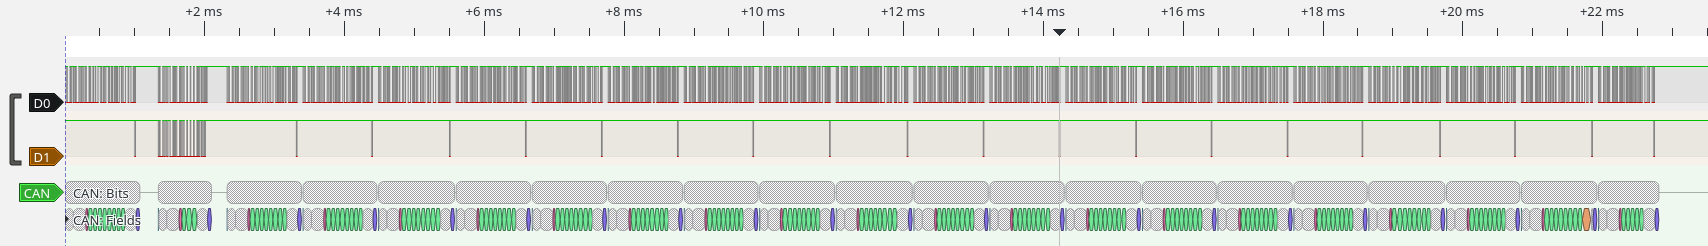
\includegraphics[width=\textwidth]{figures/eval_128_0_0.png}
        \end{center}
        \caption{UDP Transfer 128 byte, BS=0, STmin=0}
        \label{fig:udp_128_0_0}
\end{figure}

\autoref{fig:udp_128_0_0}is a capture of an UDP transfer with 128 bytes.
It uses the fastest possible parameter set with a BS of zero, which means that there are no additional FC frames to wait for and no separation time.

\begin{figure}[htp]
        \begin{center}
                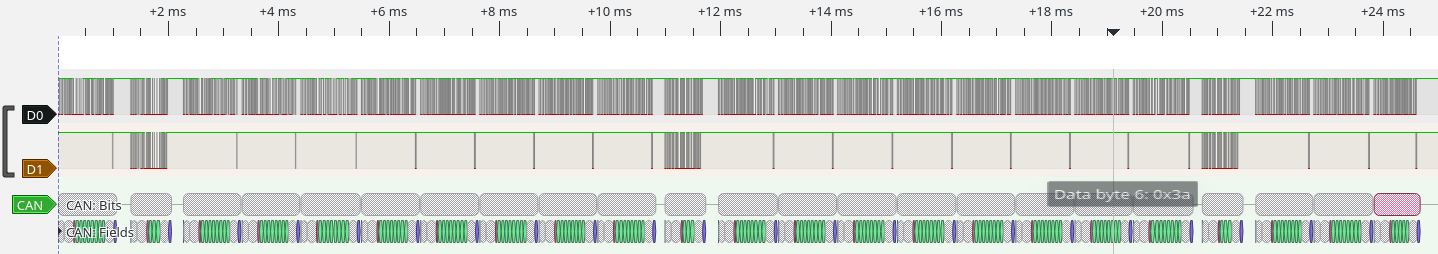
\includegraphics[width=\textwidth]{figures/eval_128_0_8.png}
        \end{center}
        \caption{UDP Transfer 128 byte, BS=8, STmin=0}
        \label{fig:udp_128_0_8}
\end{figure}

\autoref{fig:udp_128_0_8} is a capture of an UDP transfer with 128 bytes.
It uses a BS of eight, which means that every eight frames, the sender has to wait for another FC frame with a CTS state. The separation time is zero.

\begin{figure}[htp]
        \begin{center}
                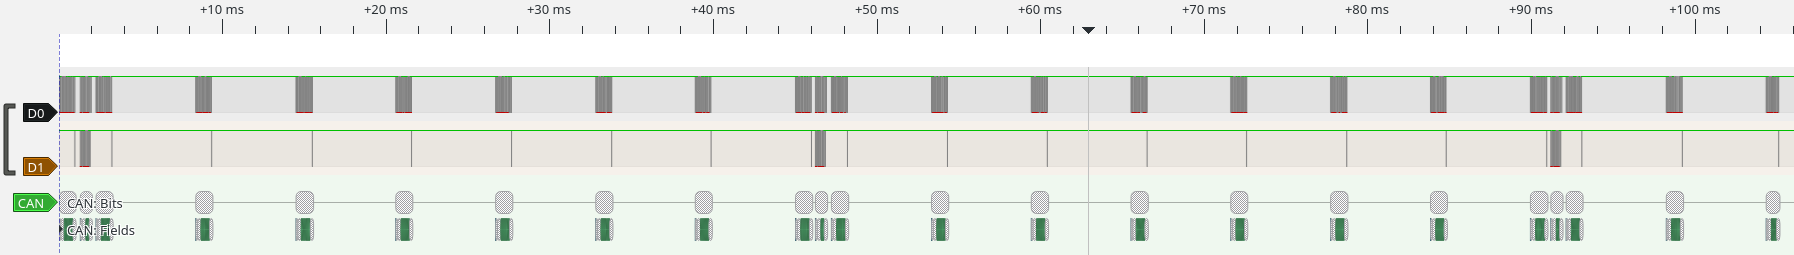
\includegraphics[width=\textwidth]{figures/eval_128_5_8.png}
        \end{center}
        \caption{UDP Transfer 128 byte, BS=8, STmin=5}
        \label{fig:udp_128_5_8}
\end{figure}

\autoref{fig:udp_128_5_8} is a capture of an UDP transfer with 128 bytes.
It shows a combination of a BS of eight and a separation time of five ms.
The separation time can, for example, be used to reduce the load on the bus.
